\section{Resultados}

% ------ estrutura
\subsection{Resultados}
	\begin{frame}\frametitle{Gerador de aleatoriedade}
		\begin{itemize}
			\item Distribuição no tempo e no espaço
			\item Controlabilidade e flexibilidade
		\end{itemize}

		\begin{figure}
			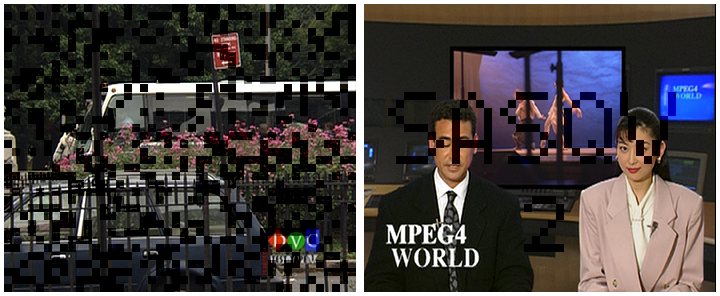
\includegraphics[width=0.8\textwidth]{./imgs/raffle.png}
			\caption{Resultados dos sorteios}
			\tiny
			Fonte: Autoria própria.
		\end{figure}
    \end{frame}

    \begin{frame}\frametitle{Blocagem}
		\begin{itemize}
			\item Diferentes níveis independentes de blocagem
			\item Janela variável
		\end{itemize}

		\begin{figure}
			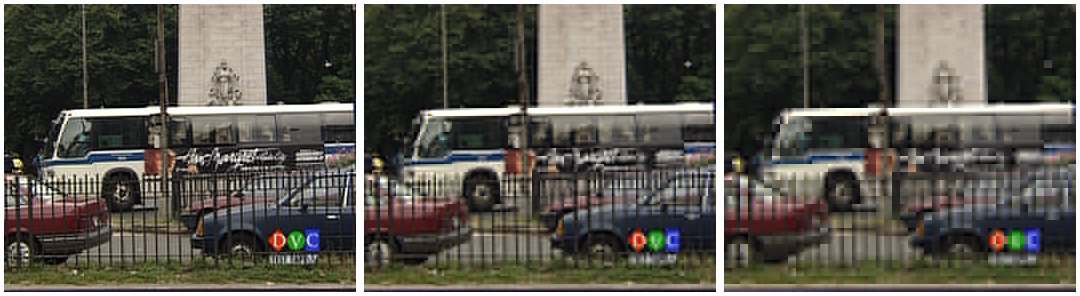
\includegraphics[width=0.8\textwidth]{./imgs/block.png}
			\caption{Resultados da blocagem}
			\tiny
			Fonte: Autoria própria.
		\end{figure}

    \end{frame}
	
	\begin{frame}\frametitle{Borramento}
		\begin{itemize}
			\item Dois tipos de filtros
			\item Janela variável
		\end{itemize}

		\begin{figure}
			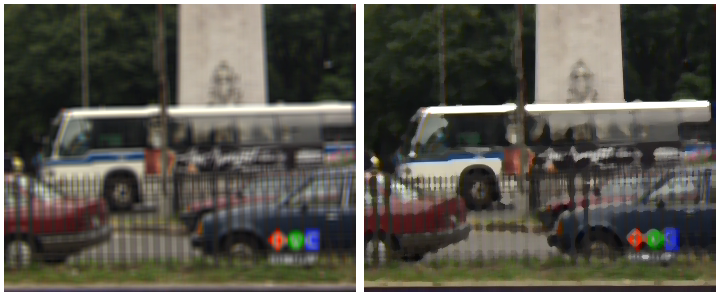
\includegraphics[width=0.8\textwidth]{./imgs/blur.png}
			\caption{Resultados do borramento}
			\tiny
			Fonte: Autoria própria.
		\end{figure}

    \end{frame}
	
	\begin{frame}\frametitle{Simulador de streaming}
		\begin{itemize}
			\item Descarte de pacotes
		\end{itemize}

		\begin{figure}
			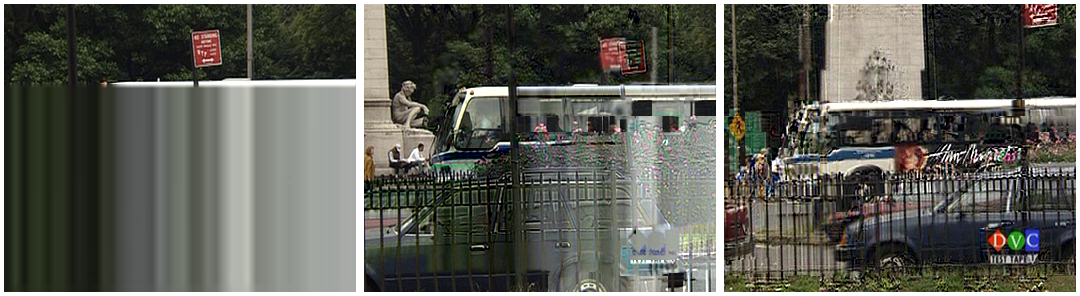
\includegraphics[width=0.8\textwidth]{./imgs/net.png}
			\caption{Resultados do simulador}
			\tiny
			Fonte: Autoria própria.
		\end{figure}

    \end{frame}
		
	\begin{frame}\frametitle{Métricas}
		\begin{itemize}
			\item MSE e PSNR: consistentes
			\item MSSIM: pequenas variações e comportamento consistente
		\end{itemize}

		\begin{table}
			\tiny
			\caption{Tabela de erros na validação}
			\begin{tabular}{lccc}
			\hline
			Video & MSE (\%) & PSNR (\%) & MSSIM (\%) \\
			\hline
			aircraft & 0.00000 & 0.00000 & 1.59306 \\
			liberty  & 0.00000 & 0.00000 & 0.24843 \\
			ship     &-0.00001 & 0.00000 & 0.23530 \\
			stockholm &0.00000 & 0.00000 & 1.97948 \\
			whale    & 0.00621 & 0.00000 & 0.39320 \\
			\hline
			\end{tabular}
			\\ ~ \\
			\tiny
			Fonte: Autoria própria.
		\end{table}
    \end{frame}
